\documentclass{beamer}
%\setbeamertemplate{navigation symbols}


\usetheme{Montpellier}

\beamersetuncovermixins{\opaqueness<1>{25}}{\opaqueness<2->{15}}
\begin{document}
\title{A quick look into verification in OS kernels}  
\author{ZEGAOUI Taquyeddine}
\date{\today} 
\begin{frame}
\titlepage
\end{frame}

\begin{frame}\frametitle{Table of contents}\tableofcontents
\end{frame} 

%-------------------------------------------------------------------------------------------------------------------------------------------------------------------------------------------------------------------------------------------------------------------------------------------------------------------------------

\section{Introduction}

\subsection{A certain kind of security threat}

\begin{frame}
What do Bitcoin transaction scripting, network packet filtering  and power management have in common ?
\\
\pause
They all make use of in-kernel interpreters !
\end{frame}

\begin{frame}\frametitle{In-kernel interpreters}
\begin{itemize}[<+->]
	\item In-kernel interpreters have become a staple of modern computation processes
	\item They also have become a major concern regarding security
	\item Risks of malicious attacks or intern errors
	\item In-kernel interpreters run in kernel space
	\item Any error or attack can have tremendous consequences
 \end{itemize}
\pause
What can be done to guarantee safe and correct in-kernel interpreters ?
\end{frame}

\begin{frame}\frametitle{A solution for in-kernel interpreters}
One way of securing an in-kernel interpreter is limiting its powers to stop it from posing a security threat. System call filtering is a great way to do this:
\begin{itemize}[<+->]
	\item System calls are THE only way to interact with the system
	\item They are well known system routines
	\item Each system call is self sufficient
	\item Each system call performs a single defined action
	\item All we need is a way to monitor and filter system calls
 \end{itemize}
\pause
So what means do we have for system call filtering ?
\end{frame}

%-------------------------------------------------------------------------------------------------------------------------------------------------------------------------------------------------------------------------------------------------------------------------------------------------------------------------------
\section{System call filtering}

\subsection{System call policies: BPF}

\begin{frame}\frametitle{What is BPF ?}
The BPF language
\begin{itemize}[<+->]
	\item Originally serves for defining packets filters
	\item Is a low-level language rather close to assembly
	\item Is used here as a system call filter
 \end{itemize}
\end{frame}

\begin{frame}[fragile, shrink]\frametitle{BPF syntax}
\begin{verbatim}
; load syscall number
ld [0]
; deny open() with errno = EACCES
jeq #SYS_open, L1, L2
L1: ret #RET_ERRNO|#EACCES
; allow getpid()
L2: jeq #SYS_getpid, L3, L4
L3: ret #RET_ALLOW
; allow gettimeofday()
L4: jeq #SYS_gettimeofday, L5, L6
L5: ret #RET_ALLOW
L6: ...
; default: kill current process
ret #RET_KILL
\end{verbatim}
\pause
As seen above, each system call gets an entry in the list of rules, along with the expected behavior regarding this particular sytem call. A default behavior is also defined, should any system call be absent from the previous list.
\end{frame}

\begin{frame}\frametitle{Inconvenients of BPF}
But BPF is relatively complex to write, and can cause mistakes or errors that can lead to incorrect system call policies.
\pause
We need an easy way to define BPF system call policies.
\end{frame}

\subsection{User-friendly rules definition: SCPL}

\begin{frame}\frametitle{Introducing SCPL}
We introduce SCPL, a domain specific language for defining sytem call policies
\begin{itemize}[<+->]
	\item In a more user-friendly way, being close to natural human language
	\item In an easier, more intuitive and less prone to errors manner
	\item Which reduces the risk of having incorrect BPF policies
	\item Which will be translated to BPF
 \end{itemize}
\end{frame}

\begin{frame}[fragile]\frametitle{Example of SCPL}
\begin{verbatim}
{ default_action = Kill;
rules = [
{ action = Errno EACCES; syscall = SYS_open };
{ action = Allow; syscall = SYS_getpid };
{ action = Allow; syscall = SYS_gettimeofday };
...
] }
\end{verbatim}
\pause
As seen above, SCPL is really close to the natural thought process of defining the rules of sytem call behavior, and this intuitive ease of use guarantees minimal errors within policies definition.
\end{frame}

\subsection{Policies enforcement: JITK}
\begin{frame}\frametitle{Use of BPF policies}
The previously defined BPF system call policies are then:
\begin{itemize}[<+->]
	\item Compiled to native code to be passed to the kernel
	\item Guaranteed to correctly translate into native code without loss of meaning
	\item Used to determine behavior regarding every sytem call
	\item Able to be checked by the interpreter without overhead cost
 \end{itemize}
\end{frame}

%-------------------------------------------------------------------------------------------------------------------------------------------------------------------------------------------------------------------------------------------------------------------------------------------------------------------------------

\section{Introducing JITK} 

\subsection{Overview of JITK}

\begin{frame}\frametitle{JITK: what is it ?}
Enter JITK,
\begin{itemize}[<+->]
	\item An infrastructure for building in-kernel interpreters
	\item Guarantees complete functional correctness
	\item Uses user-defined system call policies to secure execution
	\item Those policies define what system call the executing code can invoke
 \end{itemize}
\end{frame}

\begin{frame}\frametitle{Correctness guarantees in JITK}
Using Coq, JITK is able to guarantee correctness regarding:
\begin{itemize}[<+->]
	\item Implementation of each of its components
	\item User-space compilation of SCPL to BPF
	\item Kernel-space compilation of BPF to native code
	\item Application and enforcement of said policies
 \end{itemize}
\end{frame}

\subsection{Overview of Coq}

\begin{frame}\frametitle{Introducing Coq}
Coq
\begin{itemize}[<+->]
	\item A powerful proof assistant, written in Ocaml
	\item Able to help formally proving software
	\item Uses a form of mathematical language, called Gallina
	\item Was used to implement CompCert, a certified C2native compiler
 \end{itemize}
\end{frame}

\begin{frame}[shrink]\frametitle{Coq syntax example}
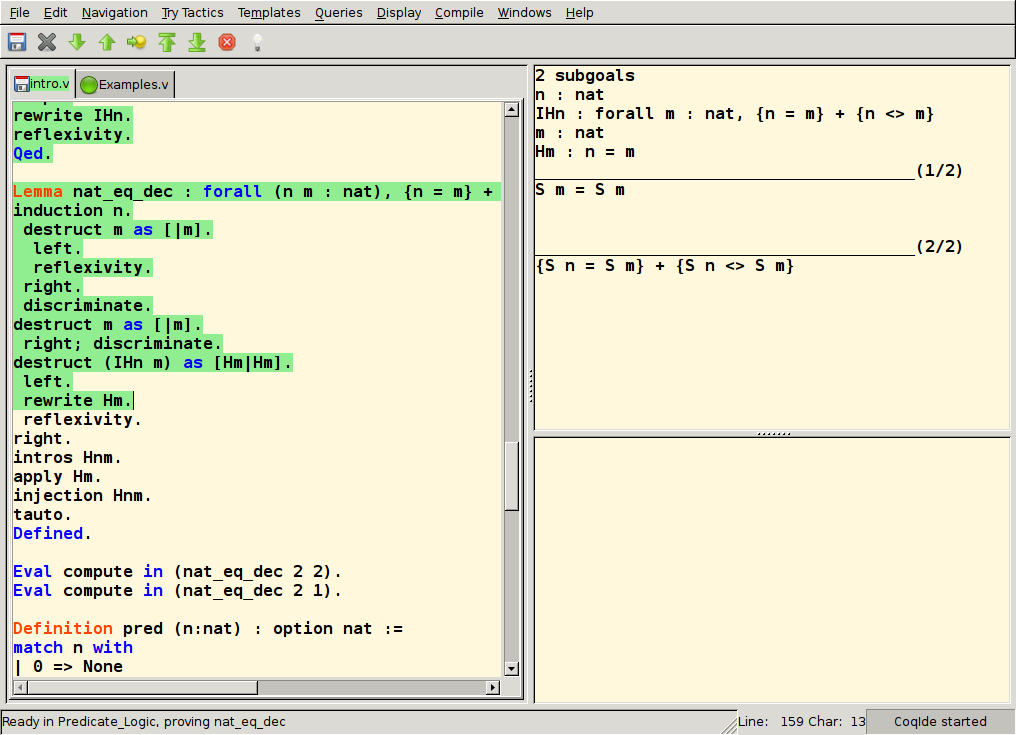
\includegraphics[scale=0.5]{CoqProof.png}
\end{frame}

\subsection{Inner workings of JITK}

\begin{frame}
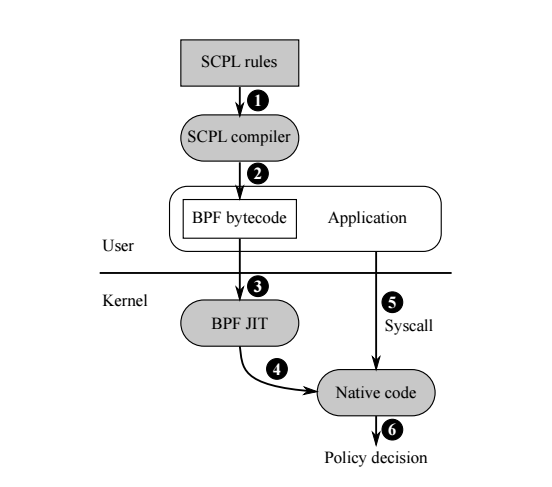
\includegraphics[scale=0.5]{Graph2.png}
\end{frame}
\begin{frame}\frametitle{JITK operation steps}
JITK operation is divided in several steps:
\begin{itemize}[<+->]
	\item User definition of SCPL rules
	\item Compilation of SCPL rules to BPF policies
	\item Encoding of BPF policies to BPF bytecode
	\item Transmission of BPF bytecode to kernel space
	\item Decoding and checking to get BPF instructions
	\item Translation to Cminor
	\item Compilation to native assembly using CompCert
	\item Validation and assembly to get native binary code
\end{itemize}
\end{frame}
\begin{frame}
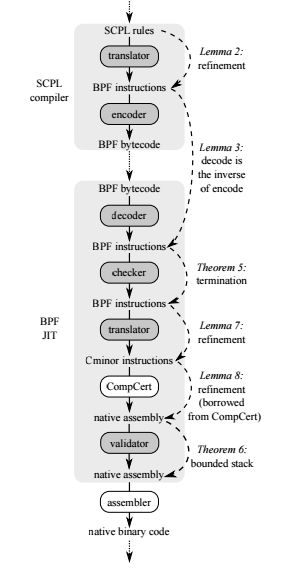
\includegraphics[scale=0.3]{Graph1.png}
\end{frame}




\section{}
\begin{frame}
Thank you for your attention ! Any questions ?
\end{frame}
\begin{frame}[allowframebreaks]
  \frametitle<presentation>{Further Reading}    
  \begin{thebibliography}{10}    
  \beamertemplatearticlebibitems
  \bibitem{}
    Xi Wang, David Lazar, Nickolai Zeldovich, Adam Chlipala, Zachary Tatlock
    \newblock Jitk: A Trustworthy In-Kernel Interpreter Infrastructure.
    \newblock 11th USENIX Symposium on Operating Systems Design and Implementation, 2014.
  \beamertemplatearticlebibitems
  \bibitem{}
    Grigore Rosu, Traian Florin Serbanuta
    \newblock An Overview of the K Semantic Framework
    \newblock J.LAP, 2010.
  \end{thebibliography}
\end{frame}


\end{document}